\documentclass[12pt,letterpaper]{article}

% Evidencia: GA4-220501095-AA2-EV04
% Compilar con LaTeX Workshop o: latexmk -pdf GA4-220501095-AA2-EV04.tex
% El contenido usa caracteres ASCII para evitar problemas de codificacion.

\usepackage[spanish,es-nodecimaldot,shorthands=off]{babel}
\usepackage[T1]{fontenc}
\usepackage[utf8]{inputenc}
\usepackage{lmodern}
\usepackage{geometry}
\usepackage{setspace}
\usepackage{array}
\usepackage{longtable}
\usepackage{enumitem}
\usepackage{xcolor}
\usepackage{titlesec}
\usepackage{fancyhdr}
\usepackage{graphicx}
\usepackage{pdflscape}
\usepackage{hyperref}

% ==================== DATOS CONFIGURABLES ====================
\newcommand{\institucion}{Servicio Nacional de Aprendizaje -- SENA}
\newcommand{\programa}{Analisis y Desarrollo de Software}
\newcommand{\tituloTrabajo}{Diagrama de clases del proyecto de software}
\newcommand{\codigoEvidencia}{GA4-220501095-AA2-EV04}
\newcommand{\nombreProyecto}{Sistema de Gestion de Citas SAC}
\newcommand{\aprendiz}{Kevin Andres Granados Daza}
\newcommand{\instructor}{[Jesus Ramirez]}
\newcommand{\ficha}{[3389015]}
\newcommand{\ciudad}{Bogota D. C.}
\newcommand{\fechaEntrega}{[25 de septiembre de 2026]}
% ==============================================================

\geometry{top=2.54cm,bottom=2.54cm,left=2.54cm,right=2.54cm}
\onehalfspacing
\setlength{\parindent}{1.27cm}
\setlength{\parskip}{0pt}
\setlength{\headheight}{15pt}

\pagestyle{fancy}
\fancyhf{}
\fancyhead[L]{\codigoEvidencia}
\fancyhead[R]{\thepage}
\renewcommand{\headrulewidth}{0pt}

\titleformat{\section}{\normalfont\Large\bfseries\centering}{\thesection.}{0.5em}{}
\titleformat{\subsection}{\normalfont\large\bfseries}{\thesubsection.}{0.5em}{}

\begin{document}

\begin{titlepage}
    \centering
    \vspace*{2.5cm}
    {\Large \tituloTrabajo\par}
    \vspace{0.8cm}
    {\large Proyecto: \nombreProyecto\par}
    \vfill
    {\large \aprendiz\par}
    \vspace{1.5cm}
    {\large \institucion\par}
    {\large \programa\par}
    \vspace{1cm}
    {\large Evidencia: \codigoEvidencia\par}
    \vspace{1cm}
    {\large Instructor(a): \instructor\par}
    {\large Ficha: \ficha\par}
    \vfill
    {\large \ciudad\par}
    {\large \fechaEntrega\par}
\end{titlepage}

\section{Introduccion}

El diagrama de clases es uno de los diagramas mas importantes del Lenguaje Unificado de Modelado, porque permite representar la estructura estatica de un sistema orientado a objetos. Mediante este diagrama se identifican las clases principales, sus atributos, operaciones y relaciones, convirtiendose en una guia para organizar el codigo fuente y la base de datos de una aplicacion.

En el presente documento se desarrolla el diagrama de clases del proyecto \nombreProyecto. El sistema tiene como finalidad centralizar el registro de usuarios, la disponibilidad de horarios, el agendamiento de citas, la administracion de solicitudes y el seguimiento de los cambios realizados sobre cada cita.

El diseno propuesto aplica principios y buenas practicas de programacion orientada a objetos. Entre ellos se encuentran la abstraccion de entidades del dominio, el encapsulamiento de atributos, la asignacion de responsabilidades claras, el uso controlado de herencia y la definicion de relaciones con multiplicidades. Estas decisiones permiten construir una solucion mas organizada, escalable y facil de mantener.

\section{Descripcion del proyecto}

\subsection{Sistema de Gestion de Citas SAC}

El Sistema de Gestion de Citas SAC es una aplicacion web orientada a mejorar la administracion de citas y horarios de atencion. La plataforma permite que los usuarios se registren, inicien sesion, consulten la disponibilidad, soliciten citas, las cancelen o las reprogramen. Por su parte, el administrador puede crear horarios, habilitarlos o deshabilitarlos, visualizar las solicitudes y confirmar, rechazar o actualizar el estado de las citas.

El sistema responde a la necesidad de disminuir procesos manuales, evitar cruces de horarios, conservar la informacion de manera persistente y ofrecer trazabilidad sobre las acciones realizadas. Para lograrlo, se identificaron entidades principales como Rol, Usuario, Administrador, Horario, Cita, HistorialCita y Notificacion.

\subsection{Objetivo del diagrama de clases}

El objetivo del diagrama de clases es representar la estructura del Sistema de Gestion de Citas SAC antes de su implementacion. El modelo permite establecer que informacion debe manejar cada clase, que operaciones puede realizar y como se relaciona con las demas entidades del sistema.

El diagrama tambien sirve como referencia para desarrollar el modelo de datos, la logica de negocio, los servicios de la API y los casos de prueba. De esta manera, se reduce la posibilidad de duplicar responsabilidades o crear relaciones incorrectas durante la construccion del software.

\section{Criterios de diseno orientado a objetos}

Para elaborar el diagrama se aplicaron criterios que ayudan a mantener un modelo claro y coherente con los principios de programacion orientada a objetos.

\begin{longtable}{|p{4cm}|p{10.5cm}|}
\hline
\textbf{Criterio} & \textbf{Aplicacion en el Sistema de Gestion de Citas SAC} \\
\hline
\endfirsthead
\hline
\textbf{Criterio} & \textbf{Aplicacion en el Sistema de Gestion de Citas SAC} \\
\hline
\endhead
\hline
\endfoot
\hline
\endlastfoot

Abstraccion & Cada clase representa una entidad relevante del problema. Por ejemplo, Cita representa una solicitud de atencion y Horario representa una franja de tiempo disponible. \\
\hline

Encapsulamiento & Los atributos se modelan como privados mediante el simbolo menos (-). Las modificaciones de datos se realizan por medio de operaciones publicas que validan las reglas del negocio. \\
\hline

Responsabilidad unica & Cada clase tiene una funcion principal. Usuario gestiona acciones del solicitante, Horario controla disponibilidad, Cita administra el ciclo de la solicitud e HistorialCita conserva los cambios realizados. \\
\hline

Herencia justificada & Administrador hereda de Usuario porque representa un tipo especializado de usuario que conserva datos comunes y agrega permisos administrativos. \\
\hline

Bajo acoplamiento & Las clases se relacionan solo cuando es necesario. Por ejemplo, Notificacion se asocia a Cita y Usuario, pero no asume funciones de administracion de horarios. \\
\hline

Alta cohesion & Los atributos y operaciones de una clase se relacionan entre si. Los metodos de Cita se enfocan en crear, confirmar, rechazar, cancelar o reprogramar solicitudes. \\
\hline

Multiplicidades claras & Las relaciones incluyen cantidades como 1, 0..1 y 0..* para expresar las reglas del dominio y evitar ambiguedades. \\
\hline

Nombres significativos & Las clases usan sustantivos que representan entidades del dominio, mientras que las operaciones usan verbos que describen una accion concreta. \\
\hline
\end{longtable}

\section{Clases identificadas}

A partir de los requisitos, casos de uso e historias de usuario del proyecto, se identificaron las siguientes clases principales.

\begin{longtable}{|p{3.2cm}|p{5.6cm}|p{5.7cm}|}
\hline
\textbf{Clase} & \textbf{Responsabilidad} & \textbf{Elementos principales} \\
\hline
\endfirsthead
\hline
\textbf{Clase} & \textbf{Responsabilidad} & \textbf{Elementos principales} \\
\hline
\endhead
\hline
\endfoot
\hline
\endlastfoot

Rol & Define el tipo de acceso y permisos generales de un usuario dentro del sistema. & idRol, nombre, descripcion y operacion para validar permisos. \\
\hline

Usuario & Representa a la persona que utiliza la aplicacion para gestionar sus propias citas. & Datos personales, credenciales, registro, inicio de sesion, agendamiento, cancelacion y reprogramacion. \\
\hline

Administrador & Representa un usuario con permisos adicionales para gestionar horarios y solicitudes. & Hereda datos de Usuario y agrega operaciones administrativas. \\
\hline

Horario & Representa una franja de atencion que puede estar disponible, ocupada, habilitada o deshabilitada. & Fecha, hora de inicio, hora de fin, disponibilidad y operaciones de control. \\
\hline

Cita & Representa una solicitud de atencion realizada por un usuario en un horario especifico. & Fecha de solicitud, estado, observacion y operaciones para gestionar el ciclo de vida de la cita. \\
\hline

HistorialCita & Registra los cambios de estado y observaciones realizadas sobre una cita. & Estado anterior, estado nuevo, fecha de cambio, observacion y usuario que realizo la accion. \\
\hline

Notificacion & Representa los mensajes enviados a un usuario por eventos relacionados con una cita. & Mensaje, fecha de envio, tipo, estado de lectura y operaciones de envio. \\
\hline

EstadoCita & Define los valores permitidos para el estado de una cita. & Pendiente, confirmada, rechazada, cancelada, reprogramada y atendida. \\
\hline
\end{longtable}

\section{Diagrama de clases UML}

El diagrama de clases representa las clases principales del sistema, sus atributos privados, metodos publicos, herencia, asociaciones, composiciones y multiplicidades. Este modelo fue elaborado mediante una herramienta TIC de diagramacion, como Draw.io, para facilitar su visualizacion y documentacion.

% INSTRUCCION:
% 1. Genera el diagrama usando el prompt preparado para Draw.io.
% 2. Exportalo como PNG con el nombre exacto: diagrama_clases_sac.png
% 3. Guarda la imagen en la misma carpeta de este archivo .tex.
% 4. Si no deseas insertar la imagen aun, comenta o elimina el bloque landscape completo.


\begin{figure}[htbp]
    \centering
    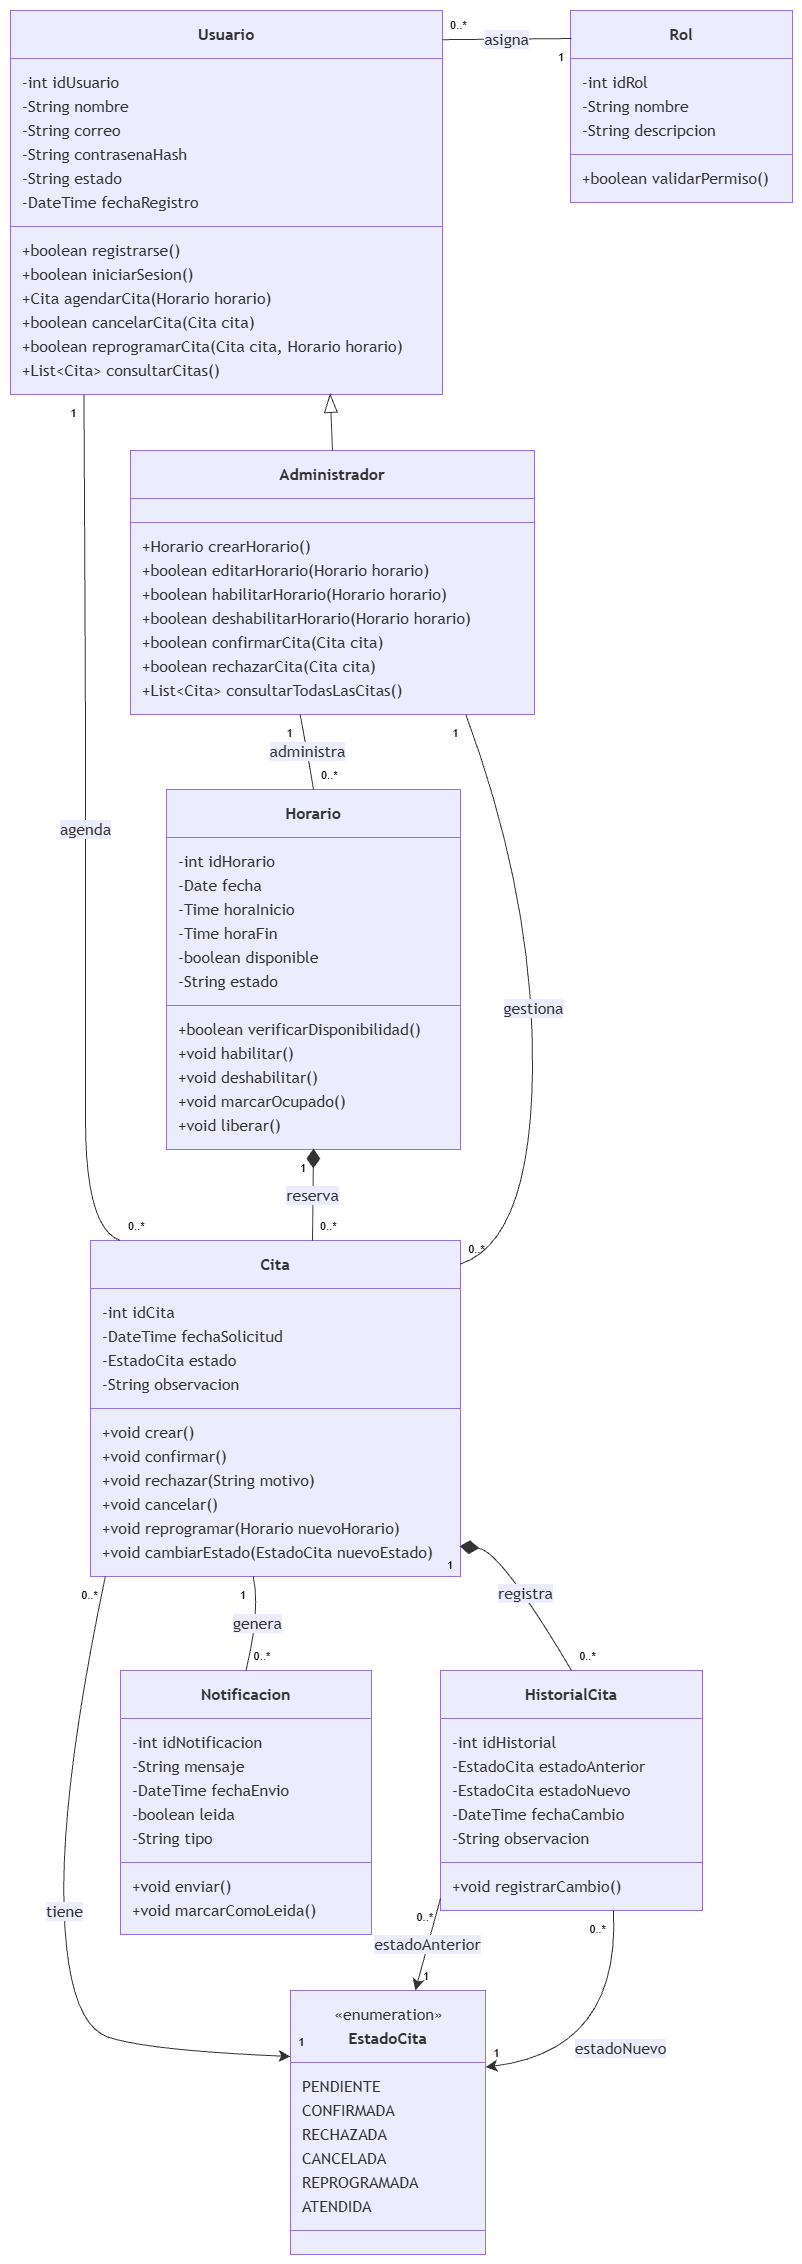
\includegraphics[width=0.45\textwidth]{diagrama_clases_sac.png}
    \caption{Diagrama de clases UML del Sistema de Gestion de Citas SAC.}
    \label{fig:diagrama-clases-sac}
\end{figure}


Como se observa en la Figura~\ref{fig:diagrama-clases-sac}, las clases se organizan de acuerdo con sus responsabilidades. Rol se relaciona con Usuario porque cada usuario debe tener un rol asignado. Administrador hereda de Usuario debido a que comparte sus datos basicos, pero incorpora operaciones adicionales para controlar los horarios y las solicitudes de cita.

La clase Cita ocupa una posicion central en el modelo, pues relaciona a un Usuario con un Horario. Cada cita utiliza un horario especifico y un horario puede estar libre o asociado a una sola cita activa. HistorialCita se modela mediante una relacion de composicion con Cita, ya que los registros de cambios dependen de la existencia de la cita a la que pertenecen. Finalmente, Notificacion se asocia con Usuario y Cita para registrar los mensajes generados por cambios importantes, como una confirmacion o cancelacion.

\section{Descripcion de relaciones y multiplicidades}

Las relaciones entre clases permiten expresar como colaboran los objetos del sistema. Las multiplicidades indican cuantos objetos pueden participar en cada relacion.

\begin{longtable}{|p{4.2cm}|p{3cm}|p{7.3cm}|}
\hline
\textbf{Relacion} & \textbf{Multiplicidad} & \textbf{Descripcion} \\
\hline
\endfirsthead
\hline
\textbf{Relacion} & \textbf{Multiplicidad} & \textbf{Descripcion} \\
\hline
\endhead
\hline
\endfoot
\hline
\endlastfoot

Rol - Usuario & 1 a 0..* & Un rol puede estar asociado a cero o muchos usuarios. Cada usuario tiene exactamente un rol asignado. \\
\hline

Usuario - Administrador & Herencia & Administrador es una especializacion de Usuario. Hereda informacion comun, como nombre, correo y credenciales, y agrega responsabilidades administrativas. \\
\hline

Administrador - Horario & 1 a 0..* & Un administrador puede crear y gestionar varios horarios. Cada horario es creado o administrado por un administrador. \\
\hline

Usuario - Cita & 1 a 0..* & Un usuario puede solicitar cero o muchas citas. Cada cita pertenece a un unico usuario. \\
\hline

Horario - Cita & 1 a 0..1 & Un horario puede estar sin cita o asociado a una sola cita activa. Cada cita utiliza un horario. \\
\hline

Cita - HistorialCita & 1 a 0..* & Una cita puede tener varios registros de historial. Cada registro de historial pertenece a una sola cita. La relacion es de composicion. \\
\hline

Usuario - HistorialCita & 1 a 0..* & Un usuario o administrador puede realizar varios cambios registrados en el historial de citas. \\
\hline

Usuario - Notificacion & 1 a 0..* & Un usuario puede recibir varias notificaciones. Cada notificacion se envia a un usuario especifico. \\
\hline

Cita - Notificacion & 1 a 0..* & Una cita puede generar varias notificaciones a lo largo de su ciclo de vida. \\
\hline

Cita - EstadoCita & Dependencia & El atributo estado de Cita utiliza los valores definidos por la enumeracion EstadoCita. \\
\hline
\end{longtable}

\section{Aplicacion de buenas practicas POO}

\subsection{Encapsulamiento}

Los atributos se representan como privados mediante el simbolo menos (-). Esto significa que no deben modificarse directamente desde cualquier parte del sistema. Por ejemplo, el estado de una cita no deberia cambiarse escribiendo directamente un nuevo valor; debe modificarse mediante operaciones como confirmar(), rechazar(), cancelar(), reprogramar() o cambiarEstado().

Esta decision permite validar las reglas del negocio antes de cambiar la informacion. Si una cita se cancela, el sistema puede liberar el horario y generar una notificacion. Si una cita se confirma, puede registrar el cambio en HistorialCita. De esta manera, la clase mantiene control sobre su propio estado.

\subsection{Herencia}

La herencia se aplica solamente entre Usuario y Administrador. Esta relacion es adecuada porque un administrador es un tipo de usuario: comparte nombre, correo, contrasena y estado, pero posee capacidades adicionales. El uso de herencia evita repetir los atributos comunes y facilita mantener una estructura organizada.

No se utiliza herencia en clases como Cita, Horario o Notificacion porque no representan tipos especializados de Usuario. En estos casos es mas adecuado usar asociaciones, ya que los objetos colaboran entre si sin que uno sea una version del otro.

\subsection{Responsabilidad unica}

Cada clase tiene una responsabilidad concreta. Usuario se enfoca en las acciones del solicitante; Administrador se encarga de tareas de control; Horario administra disponibilidad; Cita controla el ciclo de una solicitud; HistorialCita conserva cambios; y Notificacion informa eventos relevantes.

Esta separacion evita que una sola clase acumule demasiadas funciones. Por ejemplo, la clase Cita no debe encargarse de autenticar usuarios ni de crear horarios; su responsabilidad es administrar los datos y estados de una solicitud de cita.

\subsection{Asociaciones y composicion}

Se utilizan asociaciones cuando dos clases necesitan colaborar, como Usuario y Cita o Cita y Horario. Estas relaciones permiten navegar entre objetos sin convertir una clase en parte inseparable de la otra.

La composicion se utiliza entre Cita e HistorialCita. Un registro de historial no tiene sentido por si solo si la cita asociada no existe. Por esta razon, HistorialCita depende del ciclo de vida de Cita y se representa con un rombo negro en el extremo de la clase Cita.

\subsection{Enumeracion para estados}

La clase Cita utiliza la enumeracion EstadoCita para limitar los valores posibles de su atributo estado. Esta practica evita errores causados por escribir estados diferentes para una misma situacion, por ejemplo "confirmada", "confirmado" o "confirmar". Los valores permitidos se definen de forma centralizada: PENDIENTE, CONFIRMADA, RECHAZADA, CANCELADA, REPROGRAMADA y ATENDIDA.

\section{Reglas de negocio reflejadas en el diagrama}

El modelo de clases permite representar varias reglas importantes para el funcionamiento del Sistema de Gestion de Citas SAC:

\begin{itemize}[leftmargin=1.2cm]
    \item Cada usuario debe tener un rol asignado.
    \item Solamente un administrador puede crear, editar, habilitar o deshabilitar horarios.
    \item Una cita solo puede crearse si el horario seleccionado se encuentra disponible.
    \item Un horario no puede estar asociado a mas de una cita activa al mismo tiempo.
    \item Cada cita debe pertenecer a un usuario y utilizar un horario especifico.
    \item Los cambios de estado de una cita deben registrarse en HistorialCita.
    \item Una cita puede generar notificaciones cuando se crea, confirma, rechaza, cancela o reprograma.
    \item Los estados de una cita deben corresponder a uno de los valores definidos en EstadoCita.
\end{itemize}

\section{Conclusiones}

El diagrama de clases elaborado para el Sistema de Gestion de Citas SAC permite representar de forma organizada las entidades principales necesarias para implementar el proyecto. Las clases Rol, Usuario, Administrador, Horario, Cita, HistorialCita y Notificacion responden a las funciones identificadas en los requisitos y casos de uso del sistema.

La aplicacion de buenas practicas de programacion orientada a objetos fortalece el diseno propuesto. El encapsulamiento protege los datos, la herencia entre Usuario y Administrador evita duplicar informacion, la responsabilidad unica mantiene las clases enfocadas y las multiplicidades expresan claramente las reglas de relacion entre los objetos.

La clase Cita se identifica como el elemento central del modelo porque conecta al usuario con un horario y registra el estado de la solicitud. El uso de HistorialCita y Notificacion complementa el diseno al proporcionar trazabilidad y comunicacion sobre los cambios realizados durante el ciclo de vida de una cita.

En conclusion, el diagrama de clases constituye una base importante para continuar con la implementacion del Sistema de Gestion de Citas SAC. El modelo facilita la construccion del codigo fuente, el diseno de la base de datos, la definicion de servicios y la elaboracion de pruebas, manteniendo coherencia con los principios de diseno orientado a objetos.

\end{document}
